%%%%%%%%%%%%%%%%%%%%%%%%%%%%%%%%%%%%%%%%%%%%%%%%%%%%%%%%%%%%%
%% HEADER
%%%%%%%%%%%%%%%%%%%%%%%%%%%%%%%%%%%%%%%%%%%%%%%%%%%%%%%%%%%%%
\documentclass[a4paper,twoside,10pt]{article}

\usepackage[english]{babel}
\usepackage[T1]{fontenc}
\usepackage[ansinew]{inputenc}
\usepackage{lmodern}

\usepackage[affil-it]{authblk}
\usepackage{verbatim}

%% Packages for Graphics & Figures %%%%%%%%%%%%%%%%%%%%%%%%%%
\usepackage{graphicx} %%For loading graphic files

%% Math Packages %%%%%%%%%%%%%%%%%%%%%%%%%%%%%%%%%%%%%%%%%%%%
\usepackage{amsmath}
\usepackage{amsthm}
\usepackage{amsfonts}

%% Other Packages %%%%%%%%%%%%%%%%%%%%%%%%%%%%%%%%%%%%%%%%%%%
\usepackage{listings}

\lstset{emph={%  
    while, for, CoreDecomposition, TemporalCores, filter, remove, not, empty, 
		add, cutAt, in, star, if, continue, intersection, set, delete, else, return
    },emphstyle={\bfseries},
  numbers=left,
  stepnumber=1,    
  firstnumber=1,
  numberfirstline=false,
}
\renewcommand{\lstlistingname}{Algorithm}% Listing -> Algorithm

\usepackage{longtable}

\newcommand{\Deg}{\mbox{\rm{deg}}}
\newcommand{\C}{\mathcal{C}}
\newcommand{\network}{\mathcal{N}}
\newcommand{\R}{\mathbb{R}}
\newcommand{\indeg}{\mbox{\rm{indeg}}}
\newcommand{\outdeg}{\mbox{\rm{outdeg}}}



%%%%%%%%%%%%%%%%%%%%%%%%%%%%%%%%%%%%%%%%%%%%%%%%%%%%%%%%%%%%%
%% DOCUMENT
%%%%%%%%%%%%%%%%%%%%%%%%%%%%%%%%%%%%%%%%%%%%%%%%%%%%%%%%%%%%%
\begin{document}
\pagestyle{empty}


%% Title Page %%%%%%%%%%%%%%%%%%%%%%%%%%%%%%%%%%%%%%%%%%%%%%%
\title{Cores in temporal networks / Longitudinal approach to core maintenance}
\author{Vladimir Batagelj}
	\affil{Institute of Mathematics, Physics and Mechanics, Jadranska 19, 1000 Ljubljana,\\ University of Primorska, 6000 Koper}
\author{Monika Cerin\v sek}
	\affil{Abelium d.o.o. R\&D, Kajuhova 90, 1000 Ljubljana}
%\date{}
\maketitle

\pagestyle{plain}

%%%%%%%%%%%%%%%%%%%%%%%%%%%%%
%
%  Abstract
%
%%%%%%%%%%%%%%%%%%%%%%%%%%%%%

\begin{abstract}
TODO: zaenkrat enako kot na konferenci

Among many formalizations of the notion of dense subnetworks of a given network (clique, s-plexes, LS sets, lambda sets, cores, etc.) only for cores exists an efficient algorithm that can compute the result in an acceptable time also for large networks.

In a graph $G = (V, E)$ a subgraph $H = (W, E(W))$ induced by the subset of nodes $W$ is a $k$-core or a core of order $k$ iff for each node $v$ in $W$ its internal degree $\Deg_H(v)$ is greater or equal to $k$, and $H$ is a maximal subgraph with this property.

Various generalizations of ordinary cores according to types of networks and measures of node importance were proposed. In our contribution we extend the notion of cores to temporal networks and present the corresponding algorithms. For illustration we present results of determining cores in selected artificial and real-life networks.

\noindent
{\bf Keywords}: \\
{\bf Mathematics Subject Classification}:

\end{abstract}




\section{Introduction}\label{intro}
With data emerging from all aspects of our life, data analysis became our constant companion. Usage of applications is used in marketing analysis to better personalize advertisements, smart watches analyse our sleep cycle and activities to offer us recommendations for healthier life, brokers analyse stock markets to inform us about stock and cryptocurrency evaluation and value movement, etc. All this data is not constant but changes through time and time is important part of analysis. On other hand, network analysis is getting increasingly recognized not only in academic but also business sphere. Temporal network analysis enables us to better understand how relations among entities develop through time.

In this article we present new approach to the core maintenance problem in temporal network and explains it through artificial and real-life examples. Core maintenance problem is generalization of core decomposition problem in static network. With our method we search for strongly connected subgroups in a network. These groups can change through time, so we consider time to be an important part of our method.

In the next section we review the works that were the groundwork of our method and the works that contain ideas about different approach to the core maintenance problem. In Sections~\ref{definitions} we present definitions of basis concepts that lead to our method and concepts that we use in our method (temporal network, temporal core). In Section~\ref{algorithm} we present the algorithm for our method. In Section~\ref{rez} some results obtained in usage of our method of artificial and real-life data are presented.




%%%%%%%%%%%%%%%%%%%%%%%%%%%%%
%
%  Related work
%
%%%%%%%%%%%%%%%%%%%%%%%%%%%%%

\section{Related work}\label{related}

The notion of $k$-core is being used since 1983 when it was introduced by Seidman\footnote{seidman}. Let $\mathcal{G} = (\mathcal{V}, \mathcal{L})$ be a graph with set of nodes $\mathcal{V}$ and set of links $\mathcal{L}$. Let $k$ be fixed integer and let $deg(v)$ be a degree of node $v \in \mathcal{V}$. A subgraph $\mathcal{H}_k = (\C_k, \mathcal{L}|\C_k)$ induced by the subset of nodes $\C_k \subseteq \mathcal{V}$ is called a $k$-core iff $deg_{\mathcal{H}_k}(v) \geq k$, for all $v \in \C_k$, and $\mathcal{H}_k$ is maximal such subgraph. A degree of node is node property and if we replace it with another node property, we get the notion of generalized core which was introduced in \footnote{batcore}. Some other node properties are sum of incident link weights, fraction of neghbours within subset $\C$, maximal weight of incident links, etc. The node properties and restrictions on them are described in more detail in Section~\ref{definitions}.

The other possible generalization of $k$-cores is onto two-mode networks. The notion of $(p, q)$-core was introduced in \footnote{pqcore} and the notion of generalized two-mode cores was introduced in\footnote{gen2modecore}.

We introduce new approach to generalization of core onto temporal networks. 

Few approaches to core maintenance problem are already available:
\begin{itemize}
\item determine nodes that need recalculation of core number with restriction that network changes only with inserting or removing links \footnote{liyu}
\end{itemize}

Core maintenance problem was also used for communtity identification and maintenance in \footnote{community}.


TODO: ostali algoritmi za core maintenance

citiraj core1 (a fast order-based approach for core maintenance)


%%%%%%%%%%%%%%%%%%%%%%%%%%%%%
%
%  Definitions
%
%%%%%%%%%%%%%%%%%%%%%%%%%%%%%
\section{Definitions}\label{definitions}
TODO do Generalized core

Core of order $k$

Network: 
$
\mathcal{N} = (\mathcal{V}, \mathcal{L}, \mathcal{P}, \mathcal{W}); \; n = |\mathcal{V}|, m = |\mathcal{L}|$

k-core (Seidman 1983): 
A subgraph $\mathcal{H} = (\C,\mathcal{L}(\C))$ induced by the
set of nodes $\C$ is a $k$-core or a core of order $k$ iff $\forall v \in \C : deg_\mathcal{H}(v) \geq k$ and $\mathcal{H}$ is the maximum
subgraph with this property.


The core of maximum order -- main core.

The core number of node $v$ is the highest order of a core that contains this node.

\begin{figure}[!h]
	\centering
  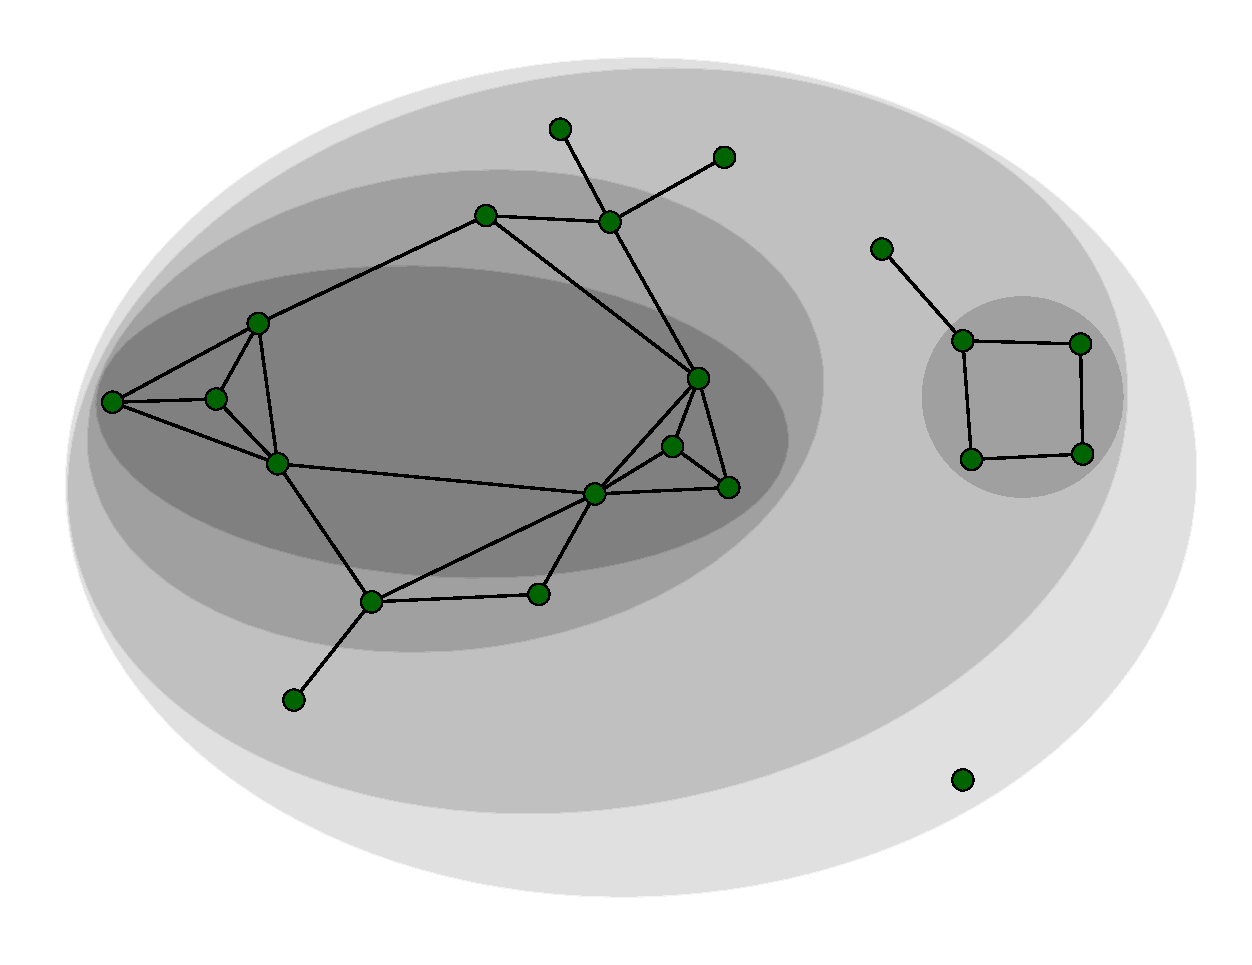
\includegraphics[width=\textwidth]{./pics/kcore.pdf}
  \caption{All $k$-cores of a network.}
  \label{kcore}
\end{figure}


\subsection{Generalized core}

Node property function $p(v, \C)$ is defined for all $v \in \mathcal{V}$
in a network $\mathcal{N} = (\mathcal{V}, \mathcal{L}, \mathcal{P}, \mathcal{W})$ and for $\C$ being a subset in $\mathcal{V}$. Function $p$ is defined as $p: L \longrightarrow \R^+$.

Let us mark $N(v)$ as a neighbourhood of a node $v$ in network $\mathcal{N}$ and $N(v, \C)$ as a neighbourhood of a node $v$ within the subset $\C$. We define node property function $p$ such that two properties hold for it:
\begin{itemize}
\item $p(v, \C)$ is local: $p(v, \C) = p(v, N(v, \C)) \; \forall v \in \mathcal{V}$.
\item $p(v, \C)$ is monotonic: $\C_1 \subset \C_2 \Rightarrow \forall v \in \mathcal{V}: p(v, \C_1) \leq p(v, \C_2).$.
\end{itemize}

Some node properties were proposed in \footnote{citiraj batcores}. Examples of node property functions are:
\begin{enumerate}
\item $p_1 (v, \C) = \Deg_{\C}(v)$: node degree within $\C$
\item $p_2 (v, \C) = \indeg_{\C}(v) + \outdeg_{\C}(v)$: if lines are directed it holds $p_2 = p_1$
\item $\mathbf{p_3 (v, \C) = \sum_{u \in N(v, \C)} w(v,u)}$ \textbf{for} $\mathbf{w: L \rightarrow \mathbb{R}_0^+:}$ \textbf{sum of weights of incident lines within $\C$}
\item $p_4 (v, \C) = \max_{u \in N(v, \C)} w(v, u)$ for $w: L \rightarrow \mathbb{R}$: maximal weight of incident lines within $\C$
\item $p_5 (v, \C) = \frac{\deg_{\C}(v)}{\deg(v)}$ if $\deg(v) > 0$ else $f_5 (v, \C) = 0$: fraction of neighbors within $\C$.
\item $p_6 (v, \C) = \frac{\sum_{u \in N(v, \C)} w(v,u)}{\sum_{u \in N(v)} w(v,u)}$ for $w: L \rightarrow \mathbb{R}_0^+$: fraction of sum of weights of incident lines within $\C$.
\end{enumerate}


With node property functions as described above authors in \footnote{citiraj batcores} defined a notion of generalized cores. 
The subgraph $\mathcal{H} = (\C,\mathcal{L}(\C))$ induced by the set $C \subseteq \mathcal{V}$ is a $p$-core at level $t \in \mathbb{R}$ iff $\forall v \in \C : t \leq f(v, \C)$ and $\C$ is maximal such set.


\subsection{Temporal network and temporal core}\label{temporal}

Temporal network $\mathcal{N_T} = (\mathcal{V}, \mathcal{L}, \mathcal{T}, \mathcal{P}, \mathcal{W})$ is obtained by attaching the time $\mathcal{T}$ to an ordinary network, where $\mathcal{T}$ is a set of time points: $t \in \mathcal{T}$ which are usually integers or reals. Nodes and links in temporal networks have temporal quantities assigned. Temporal quantity or $TQ$ is a list of triples $(s, f, v)$ and each triple determine the time interval in which node or link is active or present and its value in this time interval. Value $s$ is inclusive start time point, value $f$ is exclusive finish time point, and $v$ is a node or link value.

An example of temporal network is shown in Fig.~\ref{example}. All nodes in this network are present through whole time interval. Some links are directed -- direction is presented with an arrow. All links have value $1$ when they are present. Few links are not present through the whole time interval. For example, link from node $2$ to node $4$ is present from time point $3$ to time point $9$.

\begin{figure}[!h]
	\centering
  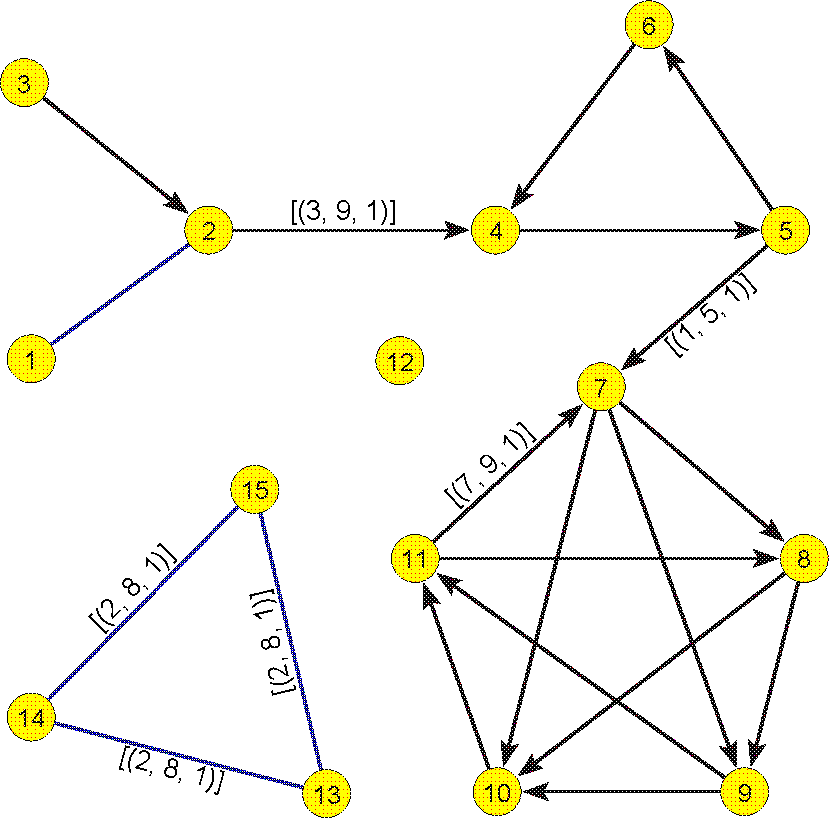
\includegraphics[width=0.7\textwidth]{./pics/Fig5.png}
  \caption{An example of a temporal network.}
  \label{example}
\end{figure}

In temporal network we assign temporal quantities to nodes and links. We use the notion of $T(v)$ being the activity set of time points for the node $v$, and $T(l)$ being the activity set of time points for the link $l$. Consistency condition must be fulfilled for activity sets: If a link $l(u, v)$ is active at the time point $t$ then its end-nodes $u$ and $v$ should be active at the time $t:$
$$T(l(u, v)) \subseteq T(u) \cap T(v).$$
\footnote{cititraj clanek Praprotnik, Batagelj}

Temporal quantity $a$ with the activity set $T_a \subseteq \mathcal{T}$ describes the changes of properties of nodes and links:
$$
a =
\begin{array}{ll}
  a'(t) & t \in T_a; \\
  undefined & t \in \mathcal{T}\backslash T_a.
\end{array}
$$

Temporal quantities allow longitudinal approach instead of time slices. An example of this approach is shown in Fig.~\ref{functions}. Temporal quantites $a$ and $b$ are shown in upper diagrams. TQ $a$ has contant value from time point $1$ to time point $4$, at time point $5$ is equal to $0$, etc. In lower diagrams are shown sum $a+b$ and multiplication $a*b$ of these temporal quantities. These operations are executed by time points -- values at a time point are summed or multiplied to get the result.

\begin{figure}[!h]
	\centering
	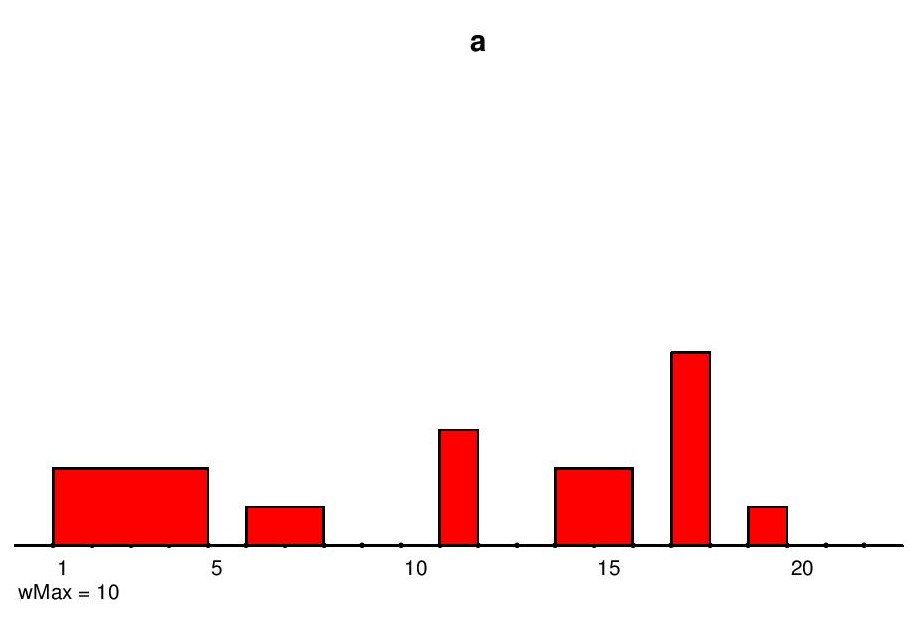
\includegraphics[width=0.45\textwidth]{./pics/a-page-001.jpg}
	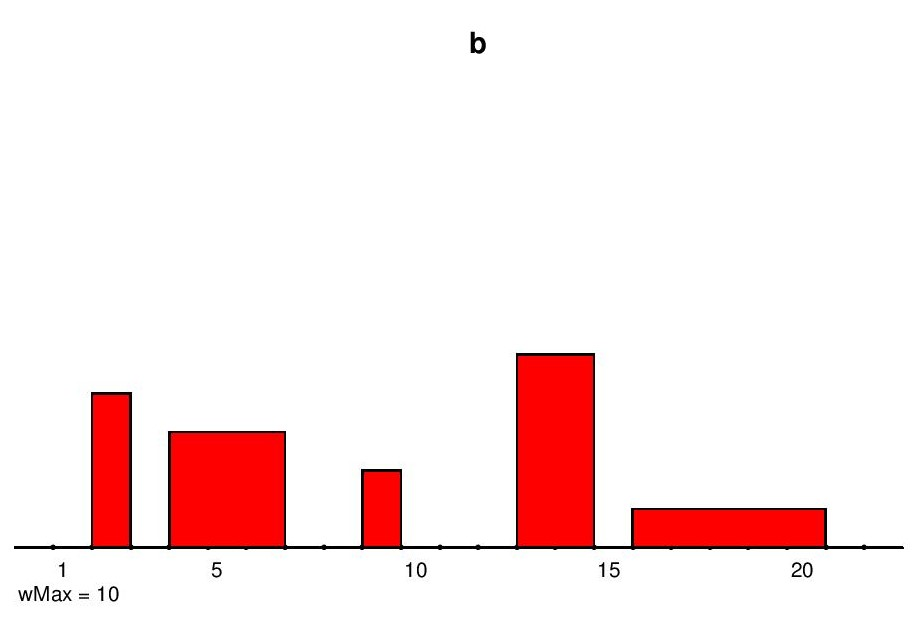
\includegraphics[width=0.45\textwidth]{./pics/b-page-001.jpg}

	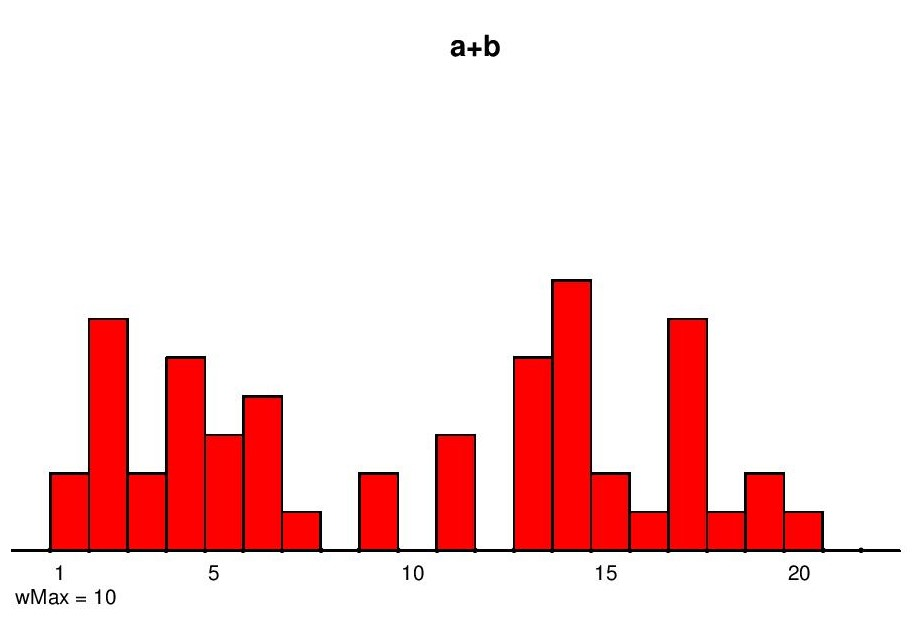
\includegraphics[width=0.45\textwidth]{./pics/sum-page-001.jpg}
	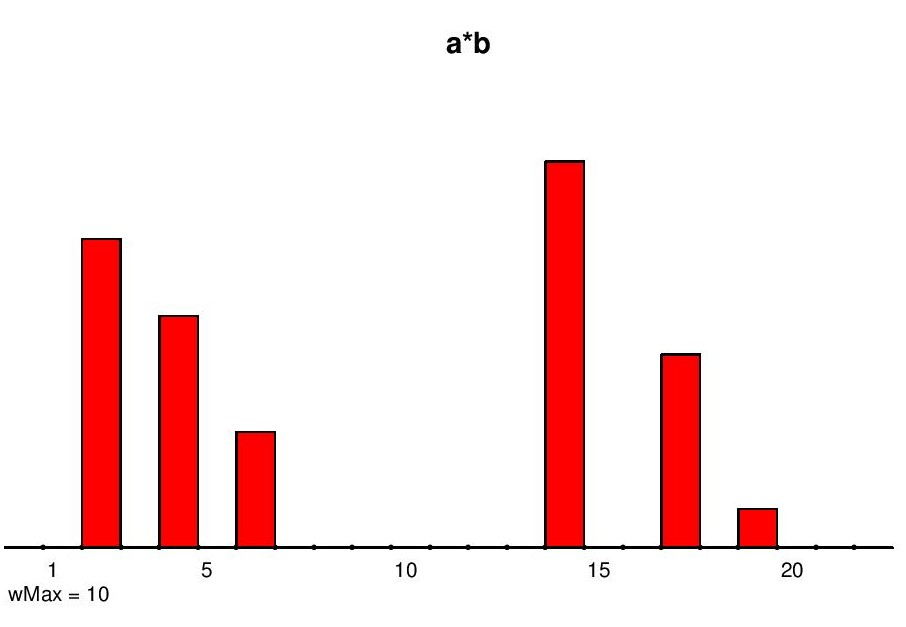
\includegraphics[width=0.45\textwidth]{./pics/pro-page-001.jpg}
  \caption{Summing and multiplying functions.}
  \label{functions}
\end{figure}


Both $k$-core and generalized core can be expanded onto temporal network. There are two main approaches to determining temporal cores -- longitudinal and with time slices. In both approaches the researcher must consider the core maintenance problem: the problem of maintaining core numbers for a temporal network. We selected longitudinal approach and based our approach on algorithm for $k$-core decomposition.




%%%%%%%%%%%%%%%%%%%%%%%%%%%%%
%
%  Algorithm
%
%%%%%%%%%%%%%%%%%%%%%%%%%%%%%
\section{The algorithm}\label{algorithm}

The algorithm for temporal core decomposition is based on algorithm for $k$-core decomposition that is presented in Alg.~\ref{coredecom}. The input for this algorithm is a network. Before main loop we copy the set of nodes into set $C$ and set a counter for core number $k$ to $1$ (lines 2 and 3 in Alg.~\ref{coredecom}). The main loop is repeated until the set $C$ contains any node. In each step we check if there exists a node in $C$ such that its degree is less than $k$. If so, we reduce degrees of its neighbours for $1$, remove the node from $C$ and set the core number of this node to $k-1.$ When no such node exists, we increase the counter $k$ for $1.$ The result is list of core numbers for all nodes of the network.

% glavni clanek
\begin{lstlisting}[mathescape, language=Python, caption={Core decomposition algorithm.}, label={coredecom}]
CoreDecomposition($\network$):
C = V
k = 1
while C $\neq \emptyset:$
	while $\exists$ u $\in$ C $\ni:$ deg(u) < k:
		for v $\in$ N(u, C):
			deg(v) = deg(v) - 1
		C = C$\backslash$v
		core(u) = k - 1
	k = k + 1
return core
\end{lstlisting}

We expanded Alg.~\ref{coredecom} onto temporal quantities and the new algorithm is shown in Alg.~\ref{alg}. Input for this algorithm is temporal network. Before main loop we copy node temporal quantities into new set $D,$ define set of core numbers for node in shape of temporal quantities, removed temporal quantities from $D$ that have a degree value equal to $0,$ and defined the dictionary $Dmin$ which consists of keys equal to nodes and values equal to minimum degree of a node. This is shown in lines 2-5 in Alg.~\ref{alg}.

The main loop (lines 6-29 in Alg.~\ref{alg}) is repeated until the set $D$ is not empty. At first we find a pair $(dmin, u)$ from $Dmin$ where $dmin$ is minimum of all values in $Dmin.$ As $core$ we define set of temporal quantities from $D[u]$ with degree equal to $dmin.$ We add these temporal quantities to the set of core numbers (line 11 in Alg.~\ref{alg}) as their degree value represent core numbers for node $u$ in given time intervals. We rewrite $core$ into  $change$ with degree values equal to $-1.$  This we need to save only those temporal quantities in $D[u]$ that have a degree larger than $dmin$ where we reduce their degrees for $1$ in those that are also in $change.$ 

Now we can check all neighbours of node $u$ -- we loop through all links of $u$ -- lines 14-25 in Alg.~\ref{alg}. If the other end-node of a link is not in $D,$ we skip it and check another link. Otherwise we define $changeLink$ as intersection of temporal quantities of a link and $change:$ time intervals are intersections of time intervals, value is equal to $-1.$ Link $changeLink$ is actually active the same time as $u$ with degree value equal to $dmin.$ If this link is never active, we skip it and check another link neighbouring $u.$ Now we define $diff$ as temporal quantities from $D[v]$ with degree value more than $0,$ where we reduce their degrees for $1$ in those that are also in $changeLink.$ Now we rewrite $D[v]$ as $diff$ with degree values equal to $\max(deg, dmin).$ If $D[v]$ is empty, we delete node $v$ from $D$ and $Dmin.$ Otherwise we set a degree value for $Dmin[v]$ to be equal to minimum degree value in $D[v].$

After checking all neighbouring links of node $u$ we check if there are any non-empty temporal quantities in $D[u]$ -- lines 26-29 in Alg.~\ref{alg}. If there are none, we delete node $u$ from $D$ and $Dmin.$ Otherwise we set a degree value for $u$ in $Dmin$ to be minimum degree value in temporal quantities of $D[u].$

\begin{lstlisting}[mathescape, language=Python, caption={Simple algorithm for cores in temporal networks.}, label={alg}]		
TemporalCores($\network$):
D = {u: [tq (start, finish, deg)]}
CoreHierarchy = {u: [tq with deg = 0]}
D = (D.filter(deg > 0)).remove(empty tq)
Dmin = {u: min deg}
while D not empty:
	(dmin, u) = (deg, u) 
			$\ni:$ (u, deg) $\in$ Dmin $\land$ deg is min deg
	core = [tq from D[u] 
			$\ni:$ deg[u] from tq is equal to dmin]
	CoreHierarchy[u].add(core)
	change = core.set(deg = -1)
	D[u] = D[u].add(change).cutAt(dmin)
	for l in $\network$.star(u):
		v = other end-node of l
		if not v in D: continue
		changeLink = l.intersection(change).
				set(deg = -1)
		if changeLink empty: continue
		diff = D[v].add(changeLink).cutAt(0)
		D[v] = diff.set(max(currentValue, dmin))
		if D[v] is empty:
			delete D[v], Dmin[v]
		else:
			Dmin[v] = tq $\in$ D[v] with min deg
	if D[u] empty:
		delete D[u], Dmin[u]
	else:
		Dmin[u] = tq $\in$ D[u] with min deg
return CoreHierarchy
\end{lstlisting}


%%%%%%%%%%%%%%%%%%%%%%%%%%%%%
%
%  Results
%
%%%%%%%%%%%%%%%%%%%%%%%%%%%%%
\section{Results}\label{rez}

We tested our method on artificial examples and examples from real-life with different context. Firstly we will look at artificial example to better understand what temporal network is and how do we determine temporal cores. 

\subsection{Artificial example}

The network is shown in Fig.~\ref{artificial1}. It consists of $15$ nodes that are always present. Most of the links are directed, some are undirected. Most of the links are present all the time -- for them there are no temporal quantities written in figure. Links $(2,4), (5,7), (11,7), (13,14), (13,15), (14,15)$ are present in defines time intervals. All links have value equal to $1$ when they are present. The degrees of nodes are listed in the left side of Tab.~\ref{artificial1tab}. For example, node $13$ has a degree equal to $0$ in time interval $[1,2)$ because both neighbouring links are not present in this time interval. In time interval $[2,8)$ are both links present, so the node has a degree equal to $2.$ After that its degree is again equal to $0,$ because no neighbouring link is present.

\begin{figure}[!h]
	\centering
	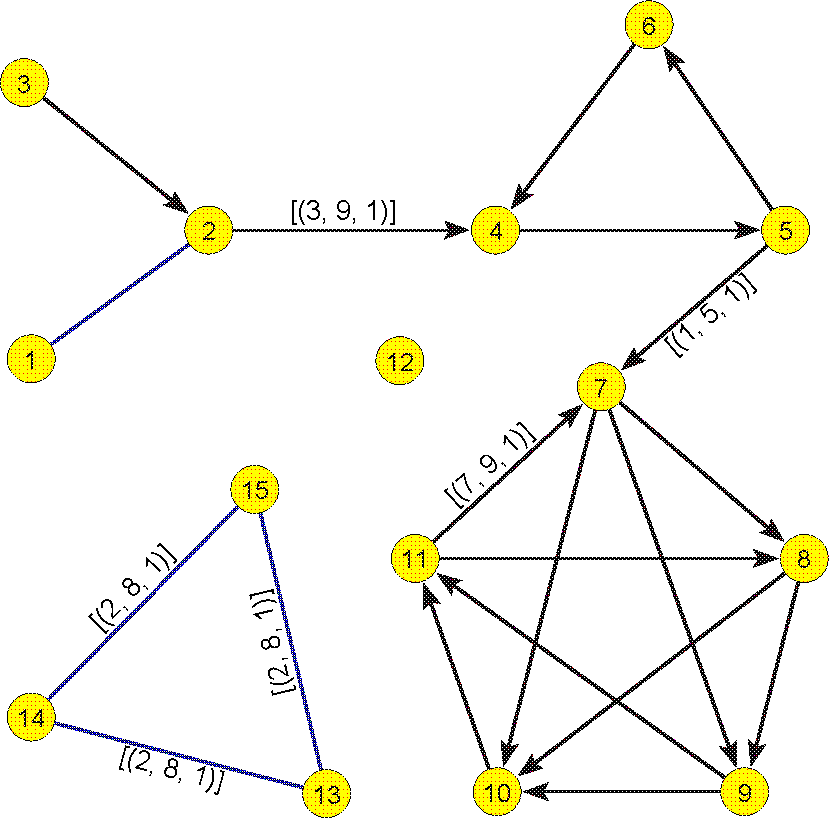
\includegraphics[width=0.7\textwidth]{./pics/Fig5.png}
  \caption{Visualization of first artificial example of a temporal network.}
  \label{artificial1}
\end{figure}

\begin{table}
\centering
\caption{Degrees and core numbers for first artificial network's nodes.}
\label{artificial1tab}
\begin{tabular}{r|l|l}
\textbf{Node} & \textbf{Degree} & \textbf{Core number} \\
\textbf{1}	&	(1, 9, 1)	&	(1, 9, 1)	\\
\textbf{2}	&	(1, 3, 2), (3, 9, 3)	&	(1, 9, 1)	\\
\textbf{3}	&	(1, 9, 1)	&	(3, 9, 1)	\\
\textbf{4}	&	(1, 3, 2), (3, 9, 3)	&	(1, 9, 2)	\\
\textbf{5}	&	(1, 5, 3), (5, 9, 2)	&	(1, 9, 2)	\\
\textbf{6}	&	(1, 9, 2)	&	(1, 9, 2)	\\
\textbf{7}	&	(1, 5, 4), (5, 7, 3), (7, 9, 4)	&	(1, 7, 3), (7, 9, 4)	\\
\textbf{8}	&	(1, 9, 4)	&	(1, 7, 3), (7, 9, 4)	\\
\textbf{9}	&	(1, 9, 4)	&	(1, 7, 3), (7, 9, 4)	\\
\textbf{10}	&	(1, 9, 4)	&	(1, 7, 3), (7, 9, 4)	\\
\textbf{11}	&	(1, 7, 3), (7, 9, 4)	&	(1, 7, 3), (7, 9, 4)	\\
\textbf{12}	&	(1, 9, 0)	&	(1, 9, 0)	\\
\textbf{13}	&	(1, 2, 0), (2, 8, 2), (8, 9, 0)	&	(1, 2, 0), (2, 8, 2), (8, 9, 0)	\\
\textbf{14}	&	(1, 2, 0), (2, 8, 2), (8, 9, 0)	&	(1, 2, 0), (2, 8, 2), (8, 9, 0)	\\
\textbf{15}	&	(1, 2, 0), (2, 8, 2), (8, 9, 0)	&	(1, 2, 0), (2, 8, 2), (8, 9, 0)
\end{tabular}
\end{table}

In the algorithm for temporal core decomposition we need to define sets $D,$ $CoreHierarchy,$ and $Dmin.$ For this examples these are:
\begin{itemize}
\item $D = \{1: [(1,9,1)], 2: [(1,3,2), (3,9,3)], ..., 15: [(1,2,0), (2,8,2), (8,9,0)]\}$
\item $CoreHierarchy = \{12: [(1,9,0)], 13: [(1,2,0), (8,9,0)], 14: [(1,2,0), \\(8,9,0)], 15: [(1,2,0), (8,9,0)]\}$
\item Remove temporal quantities with value 0 from $D$: $D = \{1: [(1,9,1)], 2: [(1,3,2), (3,9,3)], ..., 15: [(2,8,2)]\}$
\item $Dmin = \{1:1, 2:2, 3:1, 4:2, 5:2, 6:2, 7:3, 8:4, 9:4, 10:4, 11:3, 12:0, 13:0, 14:0, 15:0\}$
\end{itemize}

We determine $dmin$ from $Dmin$ to be $0$, which is first core number we calculate cores  with. The result of the algorithm is shown on the right in Tab.~\ref{artificial1tab}. Core number for node $1$ is equal 1 all the time. Core number for node $15$ is equal to $0$ in time intervals $[1,2)$ and $[8,9)$, and is equal to $2$ in time interval $[2,8)$.

We defined another artificial temporal network (Fig.~\ref{artificial2}) with the same underlying graph structure as in previous network (Fig.~\ref{artificial1}). The presence and values of links are different which is shown in Fig.~\ref{artificial2} and in values of nodes in Tab.~\ref{artificial2tab}. We selected sum of neighbouring link values as node values for this example so we can calculate p$_S$-core numbers for nodes. The result of the algorithm is shown on the right side of Tab.~\ref{artificial2tab}.

\begin{figure}[!h]
	\centering
	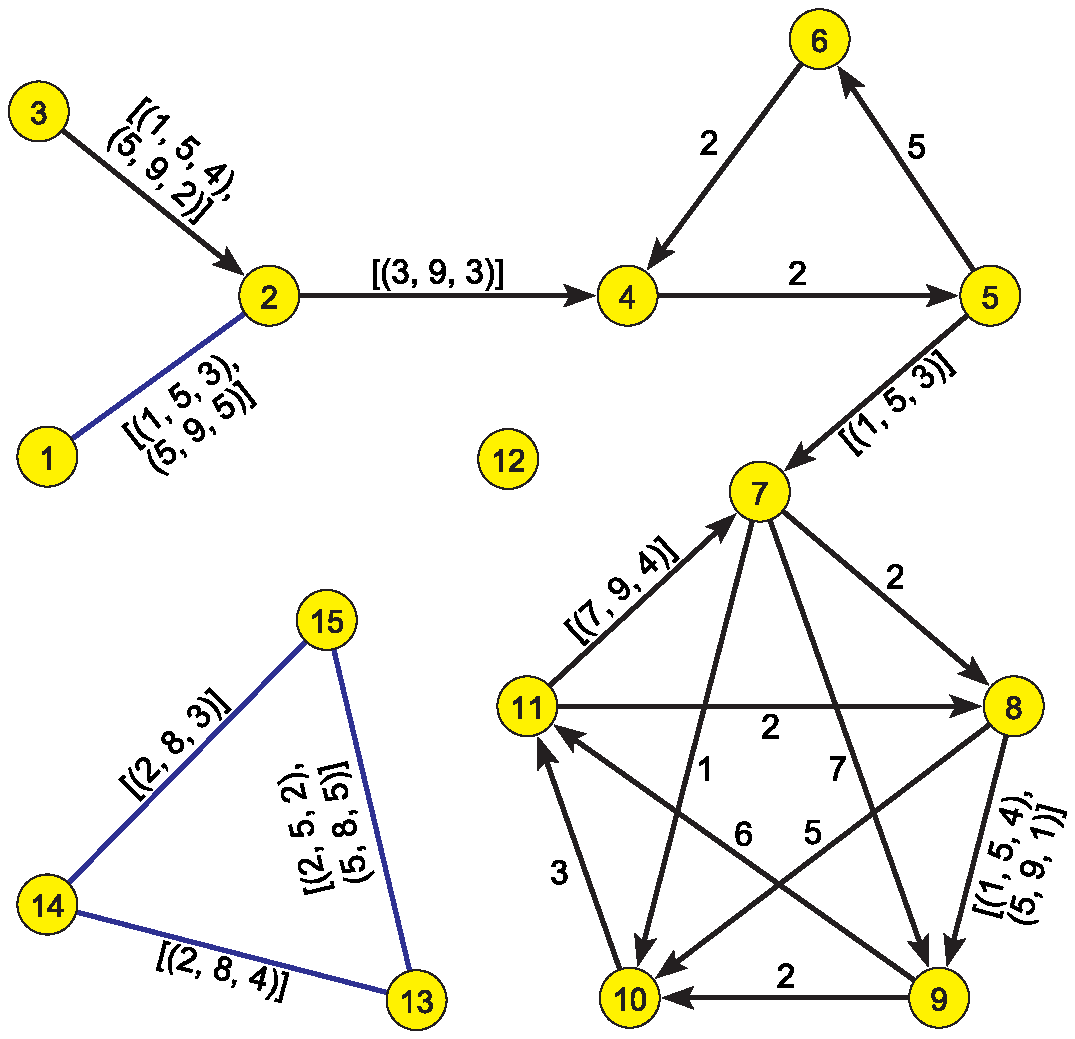
\includegraphics[width=0.7\textwidth]{./pics/connWeight.pdf}
  \caption{Visualization of second artificial example of a temporal network.}
  \label{artificial2}
\end{figure}

\begin{table}
\centering
\caption{Sums of neighbouring link values and p$_S$-core numbers for second artificial network's nodes.}
\label{artificial2tab}
\begin{tabular}{r|l|l}
\textbf{Node} & \textbf{Sum of values} & \textbf{p$_S$-core number} \\
\textbf{1}	&	(1, 5, 3), (5, 9, 5)	&	(1, 5, 3), (5, 9, 5)	\\
\textbf{2}	&	(1, 3, 7), (3, 9, 10)	&	(1, 5, 4), (5, 9, 5)	\\
\textbf{3}	&	(1, 5, 4), (5, 9, 2)	&	(1, 5, 4), (5, 9, 2)	\\
\textbf{4}	&	(1, 3, 4), (3, 9, 7)	&	(1, 5, 4), (5, 9, 5)	\\
\textbf{5}	&	(1, 5, 10), (5, 9, 7)	&	(1, 9, 5) \\
\textbf{6}	&	(1, 9, 7)	&	(1, 9, 5)	\\
\textbf{7}	&	(1, 5, 13), (5, 7, 10), (7, 9, 14)	&	(1, 9, 10)	\\
\textbf{8}	&	(1, 5, 13), (5, 9, 10)	&	(1, 9, 10)	\\
\textbf{9}	&	(1, 5, 19), (5, 9, 16)	&	(1, 9, 10)	\\
\textbf{10}	&	(1, 9, 11)	&	(1, 9, 10)	\\
\textbf{11}	&	(1, 7, 11), (7, 9, 15)	&	(1, 9, 10)	\\
\textbf{12}	&	(1, 9, 0)	&	(1, 9, 0)	\\
\textbf{13}	&	(1, 2, 0), (2, 5, 6), (5, 8, 9), (8, 9, 0)	&	(1, 2, 0), (2, 5, 5), (5, 8, 7), (8, 9, 0)	\\
\textbf{14}	&	(1, 2, 0), (2, 8, 7), (8, 9, 0)	&	(1, 2, 0), (2, 5, 5), (5, 8, 7), (8, 9, 0)	\\
\textbf{15}	&	(1, 2, 0), (2, 5, 5), (5, 8, 8), (8, 9, 0)	&	(1, 2, 0), (2, 5, 5), (5, 8, 7), (8, 9, 0)
\end{tabular}
\end{table}


\subsection{Reuters terror news network}

Data for this example was obtained from the CRA (Centering Resonance Analysis) networks produced by Steve Corman and Kevin Dooley at Arizona State University. Data is available at
 
http://vlado.fmf.uni-lj.si/pub/networks/data/CRA/terror.htm.
 
The base for this data are all stories released during $66$ consecutive days by the news agency Reuters concerning the September 11 attack on the U.S. This time interval starts at 9:00 AM EST 11th of September 2001. 

Nodes of a network are important words (terms). Two terms are connected if they appear in the same text unit (sentence). The link value is equal to the frequency of such appearances.
There are $n = 13332$ nodes and $m = 243447$ (undirected) links in a network. $50859$ of links have value more than $1$ and there are no loops.

We took $50$ most active nodes to induce a subnetwork to work with. A table representation of a such network can become quite fuzzy as can be seen in Tab.~\ref{reutersdeg}. The same goes for core numbers (Tab.~\ref{reuterscore}). We are interested in largest core numbers limited our result to only those nodes with core number at least equal to $3$. The bounded result is shown in Tab.~\ref{reuterscore3} which is more understandable than the table of all core numbers.

\begin{center}
\begin{longtable}{p{0.07\textwidth}p{0.93\textwidth}}
\caption{Degrees for nodes of induced subnetwork.}
\label{reutersdeg}\\
\textbf{Node} & \textbf{Degree} \\
\endhead
\textbf{1} & (1, 2, 5), (2, 3, 6), (3, 4, 3), (4, 5, 5), (5, 6, 4), (6, 8, 3),
     (8, 10, 5), (10, 11, 3), (11, 13, 2), (13, 16, 3), (16, 17, 4), 
     (17, 18, 5), (18, 19, 3), (19, 21, 1), (21, 22, 2), (22, 23, 1), 
     (23, 24, 4), (24, 25, 1), (25, 29, 3), (29, 31, 2), (31, 33, 3), 
     (33, 34, 1), (34, 36, 3), (36, 37, 2), (37, 39, 3), (39, 40, 4), 
     (40, 41, 2), (41, 42, 0), (42, 43, 3), (43, 44, 2), (44, 45, 3), 
     (45, 46, 1), (46, 47, 2), (47, 48, 3), (48, 49, 0), (49, 50, 4), 
     (50, 51, 1), (51, 52, 2), (52, 53, 1), (53, 54, 0), (54, 58, 2), 
     (58, 59, 3), (59, 60, 2), (60, 61, 4), (61, 62, 0), (62, 64, 2), 
     (64, 65, 1), (65, 67, 2) \\
\textbf{2} & (1, 2, 27), (2, 3, 29), ..., (63, 64, 2), (64, 65, 0), (66, 67, 0) \\
\textbf{...} & \\
\textbf{50} & (1, 2, 3), (2, 3, 2), (3, 5, 1), (5, 8, 0), (8, 10, 1), (10, 11, 2), 
     (11, 12, 1), (12, 15, 0), (15, 16, 3), (16, 17, 1), (17, 19, 0), 
     (19, 20, 1), (20, 21, 2), (21, 22, 0), (22, 24, 1), (24, 26, 0), 
     (26, 27, 2), (27, 28, 0), (28, 29, 1), (29, 31, 0), (31, 32, 1), 
     (32, 33, 0), (33, 35, 1), (35, 37, 0), (37, 38, 1), (38, 42, 0), 
     (43, 44, 2), (44, 49, 0), (49, 50, 2), (51, 57, 0), (58, 61, 0), 
     (61, 62, 1), (62, 67, 0)
\end{longtable}
\end{center}

\pagebreak
\begin{center}
\begin{longtable}{p{0.07\textwidth}p{0.93\textwidth}}
\caption{Core numbers for nodes of induced subnetwork.}
\label{reuterscore}\\
\textbf{Node} & \textbf{Core number} \\
\endhead
\textbf{1} & (1, 2, 4), (2, 3, 5), (3, 5, 3), (5, 6, 4), (6, 8, 3), (8, 10, 4), 
     (10, 11, 3), (11, 14, 2), (14, 18, 3), (18, 19, 2), (19, 21, 1), 
     (21, 22, 2), (22, 23, 1), (23, 24, 3), (24, 25, 1), (25, 28, 2), 
     (28, 29, 3), (29, 33, 2), (33, 34, 1), (34, 38, 2), (38, 39, 3), 
     (39, 41, 2), (41, 42, 0), (42, 45, 2), (45, 46, 1), (46, 47, 2), 
     (47, 48, 3), (48, 49, 0), (49, 50, 3), (50, 51, 1), (51, 52, 2), 
     (52, 53, 1), (53, 54, 0), (54, 57, 2), (57, 58, 1), (58, 59, 2), 
     (59, 60, 1), (60, 61, 2), (61, 62, 0), (62, 64, 2), (64, 65, 1), 
     (65, 67, 2) \\
\textbf{2} & (1, 3, 5), (3, 6, 4), (6, 7, 5), ..., (63, 64, 1), (64, 65, 0), (66, 67, 0) \\
\textbf{...} & \\
\textbf{50} & (1, 3, 2), (3, 5, 1), (5, 8, 0), (8, 10, 1), (10, 11, 2), (11, 12, 1),
     (12, 15, 0), (15, 16, 3), (16, 17, 1), (17, 19, 0), (19, 20, 1), 
     (20, 21, 2), (21, 22, 0), (22, 24, 1), (24, 26, 0), (26, 27, 1), 
     (27, 28, 0), (28, 29, 1), (29, 31, 0), (31, 32, 1), (32, 33, 0), 
     (33, 35, 1), (35, 37, 0), (37, 38, 1), (38, 42, 0), (43, 44, 1), 
     (44, 49, 0), (49, 50, 2), (51, 57, 0), (58, 61, 0), (61, 62, 1), 
     (62, 67, 0)
\end{longtable}
\end{center}

When we check the temporal component of the result, we found out that temporal cores of order at least $3$ appeared in first $11$ days and on day $30$. This is consistent with the idea that the news dies out with passing time.


\begin{center}
\begin{longtable}{p{0.03\textwidth}p{0.21\textwidth}p{0.76\textwidth}}
\caption{Nodes with core numbers at least equal to $3.$}
\label{reuterscore3}\\
\multicolumn{2}{l}{\textbf{Node}} & \textbf{Core number} ($\geq 3$)  \\
\endhead
1 & united\_states	& (1, 2, 4), (2, 3, 5), (5, 6, 4), (8, 10, 4) \\
2 & attack			& (1, 3, 5), (3, 6, 4), (6, 7, 5), (7, 10, 4), (11, 12, 4), (30, 31, 4)\\
4 & people         	& (1, 3, 5), (3, 6, 4), (6, 7, 5), (7, 8, 4) \\
5 & afghanistan   	&    (1, 3, 4), (5, 6, 4), (6, 7, 5), (8, 10, 4), (30, 31, 4) \\
6 & bin\_laden   	&     (1, 4, 4), (5, 6, 4), (6, 7, 5), (7, 10, 4), (11, 12, 4) \\
7 & new\_york  		&      (1, 3, 5), (3, 6, 4), (6, 7, 5), (30, 31, 4) \\
8 & pres\_bush  	&       (1, 3, 5), (3, 6, 4), (6, 7, 5), (7, 10, 4), (11, 12, 4) \\
9 & washington		&        (1, 3, 5), (3, 6, 4), (6, 7, 5), (7, 10, 4), (11, 12, 4) \\
10 & official		&          (1, 3, 5), (3, 4, 4), (5, 6, 4), (6, 7, 5) \\
12 & military       & (1, 2, 4), (5, 6, 4), (30, 31, 4)  \\
13 & plane          &  (1, 3, 5), (3, 7, 4) \\
14 & world\_trade\_ctr	&   (1, 3, 5), (3, 6, 4), (6, 7, 5), (30, 31, 4) \\
15 & security      	&    (1, 2, 4), (2, 3, 5), (5, 6, 4) \\
16 & american     	&     (2, 3, 4) \\
17 & country     	&      (1, 3, 4), (5, 10, 4) \\
18 & city       	&       (1, 3, 5), (3, 4, 4) \\
19 & war       		&        (1, 2, 4), (2, 3, 5), (5, 8, 4) \\
20 & tuesday  		&         (1, 3, 5), (3, 7, 4) \\
21 & pentagon		&          (1, 3, 5), (3, 4, 4), (5, 6, 4), (6, 7, 5) \\
22 & force  		&           (5, 6, 4) \\
23 & government     & (1, 3, 4), (5, 6, 4) \\
24 & leader        	&  (1, 4, 4), (6, 10, 4) \\
25 & world          &   (1, 3, 5), (3, 10, 4) \\
26 & terrorism     	&    (2, 3, 4) \\
27 & day          	&     (2, 3, 4), (5, 6, 4) \\
28 & week        	&      (5, 6, 4), (6, 7, 5), (8, 10, 4), (11, 12, 4) \\
29 & worker     	&       (1, 2, 4), (2, 3, 5) \\
30 & office    		&        (1, 3, 4) \\
31 & group    		&         (2, 3, 4), (6, 7, 4) \\
32 & air     		&          (2, 3, 4), (5, 6, 4) \\
34 & time   		&           (1, 3, 5), (3, 4, 4), (5, 6, 4), (7, 8, 4) \\
35 & hijack			&            (2, 3, 4) \\
36 & strike         & (2, 3, 4), (5, 6, 4), (6, 7, 5), (30, 31, 4) \\
38 & flight         &  (2, 3, 4) \\
39 & tell           &   (2, 3, 4) \\
40 & terrorist     	&    (1, 3, 4), (6, 7, 4) \\
41 & airport      	&     (2, 3, 4) \\
42 & pakistan    	&      (2, 3, 4), (5, 7, 4) \\
43 & tower      	&       (1, 3, 5), (3, 4, 4), (6, 7, 5) \\
45 & new       		&        (2, 3, 4) \\
47 & wednesday		&         (2, 3, 5), (3, 4, 4), (8, 10, 4) \\
48 & nation  		&          (1, 3, 4), (5, 6, 4) \\
49 & police 		&		            (2, 4, 4), (5, 6, 4)
\end{longtable}
\end{center}

We calculated also p$_S$-core numbers and the the result bounded to values at least equal to $20$ sre listed in Tab.~\ref{reuterscore20}. The list of nodes is almost the same as in Tab.~\ref{reuterscore3}, but time span of these cores is wider, not limited mostly to first $11$ days. The max p$_S$-core numbers through time interval is shown in Fig.~\ref{reuters}. It drops rapidly after six days which is also consistent with the idea of news getting old with passing time.

\begin{center}
\begin{longtable}{p{0.03\textwidth}p{0.2\textwidth}p{0.77\textwidth}}
\caption{Nodes with $p_S$-core numbers at least equal to $20.$}
\label{reuterscore20}\\
 \multicolumn{2}{l}{\textbf{Node}} & \textbf{p$_S$-core number} ($\geq 20$)\\
 \endhead
1 & united\_states&(1, 2, 86), (2, 3, 71), (3, 4, 34), (4, 5, 29), (5, 6, 50), (6, 7, 47), (7, 8, 22), (15, 16, 23), (18, 19, 23), (27, 28, 23)\\
2 & attack       &(1, 3, 86), (3, 4, 44), (4, 5, 36), (5, 6, 66), (6, 7, 47), (7, 8, 22), (8, 9, 21), (9, 10, 24), (10, 11, 22), (11, 12, 24), (15, 16, 23), (18, 19, 20), (27, 28, 23)\\
  3 & taliban      &(2, 3, 28), (6, 7, 20), (15, 16, 23), (27, 28, 23)\\
  4 & people       &(1, 2, 48), (2, 3, 52), (3, 4, 28), (4, 5, 32), (5, 6, 29), (6, 7, 34), (18, 19, 20)\\
  5 & afghanistan  &(1, 2, 22), (2, 3, 28), (5, 6, 29), (6, 7, 21), (15, 16, 23), (27, 28, 23)\\
  6 & bin\_laden    &(1, 2, 22), (2, 3, 28), (3, 4, 20), (5, 6, 29), (6, 7, 21), (18, 19, 20)\\
7 & new\_york     &(1, 2, 101), (2, 3, 86), (3, 4, 42), (4, 5, 35), (5, 6, 66), (6, 7, 47), (8, 9, 21), (9, 10, 24), (10, 11, 22), (11, 12, 24), (15, 16, 23), (18, 19, 20)\\
  8 & pres\_bush    &(1, 2, 48), (2, 3, 44), (5, 6, 29), (6, 7, 21)\\
9 & washington   &(1, 2, 80), (2, 3, 61), (3, 4, 27), (4, 5, 28), (5, 6, 66), (6, 7, 47), (8, 9, 21), (9, 10, 24), (10, 11, 22), (11, 12, 24), (15, 16, 23), (18, 19, 20)\\
 10 & official     &(1, 2, 40), (2, 3, 54), (3, 4, 34), (5, 6, 29), (6, 7, 36), (18, 19, 23)\\
 12 & military     &(1, 2, 25), (2, 3, 42), (5, 6, 26), (15, 16, 23), (18, 19, 23), (27, 28, 23)\\
  13 & plane        &(1, 3, 86), (3, 4, 44), (4, 5, 32), (5, 6, 50), (6, 7, 34)\\
14 & world\_trade\_c&(1, 2, 101), (2, 3, 86), (3, 4, 44), (4, 5, 35), (5, 6, 66), (6, 7, 47), (8, 9, 20), (9, 10, 21), (10, 11, 22), (11, 12, 24), (15, 16, 23), (18, 19, 20)\\
 15 & security     &(1, 2, 25), (2, 3, 30), (5, 6, 24)\\
 16 & american     &(1, 2, 48), (2, 3, 30), (5, 7, 20)\\
 17 & country      &(1, 2, 24), (2, 3, 31), (5, 6, 26), (18, 19, 20)\\
  18 & city         &(1, 2, 60), (2, 3, 52), (3, 4, 22)\\
   19 & war          &(2, 3, 34), (5, 6, 29)\\
 20 & tuesday      &(1, 3, 86), (3, 4, 44), (4, 5, 36), (5, 6, 66), (6, 7, 47)\\
21 & pentagon     &(1, 3, 86), (3, 4, 44), (4, 5, 32), (5, 6, 66), (6, 7, 47), (8, 9, 20), (9, 10, 21), (10, 11, 22), (11, 12, 24), (15, 16, 23), (18, 19, 20)\\
 22 & force        &(5, 6, 26)\\
 23 & government   &(1, 2, 28), (2, 3, 36)\\
  24 & leader       &(1, 2, 22)\\
 25 & world        &(1, 2, 34), (2, 3, 44), (18, 19, 20)\\
  26 & terrorism    &(5, 6, 20)\\
 27 & day          &(1, 2, 21), (2, 3, 36), (5, 6, 20)\\
28 & week         &(5, 6, 35), (6, 7, 27), (7, 8, 22), (8, 9, 21), (9, 10, 24), (10, 11, 22), (11, 12, 24)\\
 29 & worker       &(1, 2, 24)\\
 30 & office       &(1, 2, 34), (2, 3, 20)\\
  31 & group        &(2, 3, 26)\\
 32 & air          &(2, 3, 34), (5, 6, 29), (27, 28, 23)\\
  34 & time         &(2, 3, 36)\\
 35 & hijack       &(1, 2, 67), (2, 3, 86), (3, 4, 44), (4, 5, 28), (5, 6, 50), (6, 7, 34)\\
 36 & strike       &(2, 3, 29), (5, 6, 29), (18, 19, 22), (27, 28, 23)\\
  38 & flight       &(1, 2, 25), (2, 3, 52), (4, 5, 20)\\
   40 & terrorist    &(1, 2, 40), (2, 3, 29)\\
  41 & airport      &(1, 2, 25), (2, 3, 44), (4, 5, 25), (5, 6, 24)\\
   42 & pakistan     &(5, 6, 29)\\
 43 & tower        &(1, 2, 101), (2, 3, 72), (3, 4, 41), (4, 5, 32), (5, 6, 38), (6, 7, 32)\\
  44 & bomb         &(1, 2, 23)\\
 45 & new          &(2, 3, 30)\\
  46 & buildng      &(1, 2, 34), (2, 3, 44)\\
   47 & wednesday    &(2, 3, 52)\\
 48 & nation       &(1, 2, 31), (2, 3, 38), (5, 6, 23)\\
 49 & police       &(2, 3, 20)
\end{longtable}
\end{center}


\begin{figure}[!h]
	\centering
	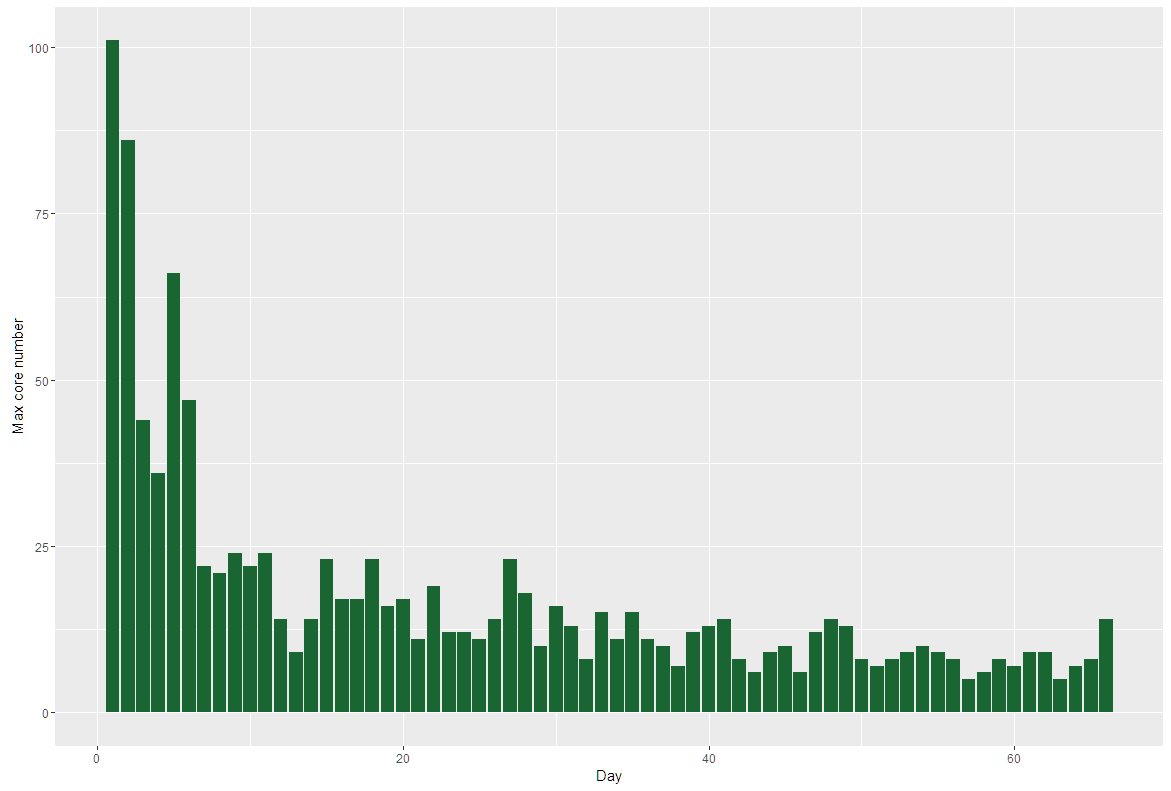
\includegraphics[width=\textwidth]{./pics/terrorMaxPSCore.png}
  \caption{Maximum $p_S$-core numbers by days from the event.}
  \label{reuters}
\end{figure}


\subsection{Stem cell research}\footnote{citiraj stembib; dodaj še vec podatkov o podatkih - recimo casovno obdobje}

A data set on the stem cell research during 1997-2012 in Spain was collected by Gisela Cantos-Mateos. A data set consists of data on papers about stem cell research in the SCI (Science Citation Index).

A network consists of $n = 577$ nodes, representing Spanish institutions, and $m = 8578$ links, representing collaborations between institutions.

Core number represents size of a group of more collaborative institutions in which a node is included. Nodes with temporal core numbers at least equal to $20$ are listed in Tab.~\ref{stemcellcore20}.

\begin{center}
\begin{longtable}{rll}
\caption{Nodes with core numbers at least equal to $20.$}
\label{stemcellcore20}\\
 \multicolumn{2}{l}{\textbf{Node}} & \textbf{Core number} ($\geq 20$) \\
 \endhead
  2 & HCSC/M      & (2010, 2011, 20), (2011, 2012, 21) \\
	3 & IN/A        & (2008, 2009, 25) \\
  5 & CIC-IBMCC/SA& (2010, 2011, 20), (2011, 2013, 22) \\
  6 & HUS/SA      & (2008, 2009, 25), (2010, 2011, 20), (2011, 2012, 21), (2012, 2013, 22)\\
  8 & IDIBELL/B   & (2011, 2012, 20) \\
  9 & UB/B        & (2008, 2009, 25), (2010, 2011, 20), (2011, 2013, 22) \\
 10 & UNIZAR/Z    & (2008, 2009, 21), (2012, 2013, 21) \\
 11 & USAL/SA     & (2008, 2009, 25), (2010, 2011, 20), (2011, 2013, 22) \\
 12 & HVH/B       & (2010, 2011, 20), (2011, 2013, 22) \\
 13 & HNJ/M       & (2010, 2011, 20), (2012, 2013, 22) \\
 16 & ICO/CT      & (2008, 2009, 25), (2010, 2011, 20), (2012, 2013, 22) \\
 17 & HMM/MU      & (2011, 2012, 22) \\
259 & HMS/Z       & (2011, 2012, 21) \\
 20 & UPC/B       & (2011, 2012, 21), (2012, 2013, 22) \\
 21 & ICREA/B     & (2010, 2011, 20) \\
 22 & HDM/B       & (2008, 2009, 21), (2012, 2013, 22) \\
 23 & UNAV        & (2008, 2009, 25), (2011, 2013, 22) \\
 24 & UPV-EHU     & (2008, 2009, 21), (2010, 2011, 20) \\
 27 & HISC3/M     & (2008, 2009, 25), (2010, 2011, 20), (2011, 2013, 22) \\
543 & PFIZER/M    & (2011, 2012, 21) \\
 32 & HRYC/M      & (2008, 2009, 21), (2010, 2011, 20), (2011, 2013, 22) \\
289 & HJXXIII/T   & (2008, 2009, 25) \\
 34 & HCL/V       & (2010, 2011, 20), (2011, 2013, 22) \\
 35 & HUGTIP/B    & (2010, 2011, 20), (2012, 2013, 20) \\
 36 & UAB/B       & (2008, 2009, 21), (2010, 2011, 20), (2011, 2013, 22) \\
 37 & US/SE       & (2010, 2011, 20) \\
 38 & UV/V        & (2008, 2009, 25), (2010, 2011, 20), (2011, 2013, 22) \\
 40 & HCL/B       & (2010, 2011, 20), (2011, 2013, 22) \\
 46 & IDIBAPS/B   & (2008, 2009, 21), (2010, 2011, 20), (2011, 2013, 22) \\
 48 & HSCSP/B     & (2008, 2009, 21), (2010, 2011, 20), (2011, 2013, 22) \\
 51 & HBST/B      & (2008, 2009, 25), (2011, 2012, 21) \\
 53 & H12O/M      & (2008, 2009, 25), (2011, 2013, 21) \\
 54 & CNB         & (2012, 2013, 22) \\
 55 & HUPH/M      & (2011, 2012, 21), (2012, 2013, 22) \\
 57 & HCLB/Z      & (2011, 2012, 21) \\
 58 & HCUN/NA     & (2011, 2013, 22) \\
266 & URL/B       & (2012, 2013, 22) \\
 62 & UAM/M       & (2008, 2009, 25), (2010, 2011, 20), (2011, 2013, 22) \\
 63 & UCM/M       & (2008, 2009, 25), (2010, 2011, 20), (2011, 2013, 22) \\
 65 & HRS/CO      & (2012, 2013, 21) \\
 66 & HCRUCES/BI  & (2011, 2012, 21) \\
 67 & CIPF/V      & (2008, 2009, 21) \\
 69 & UMA/MA      & (2008, 2009, 21), (2010, 2011, 20), (2011, 2012, 21), (2012, 2013, 22)\\
 72 & HUMV/S      & (2008, 2009, 25), (2011, 2013, 22) \\
 73 & UGR/GR      & (2011, 2012, 22), (2012, 2013, 20) \\
 74 & CIBERDEM    & (2008, 2009, 25) \\
 75 & SEHH        & (2011, 2012, 21), (2012, 2013, 20) \\
 76 & HULP/M      & (2008, 2009, 25), (2010, 2011, 20), (2011, 2013, 22) \\
 77 & UPV/V       & (2008, 2009, 21) \\
336 & TERCEL      & (2008, 2009, 25) \\
 81 & HVA/MU      & (2011, 2012, 20), (2012, 2013, 21) \\
 82 & UM/MU       & (2008, 2009, 25) \\
 85 & UA/A        & (2008, 2009, 25), (2011, 2012, 20) \\
 87 & HUP/M       & (2011, 2013, 22) \\
344 & HSO/M       & (2011, 2012, 21) \\
 89 & UPF/B       & (2008, 2009, 21), (2012, 2013, 22) \\
 91 & CIBERNED    & (2012, 2013, 22) \\
 92 & GENYO/GR    & (2011, 2012, 21) \\
 93 & CBMSO/M     & (2010, 2011, 20), (2011, 2012, 22), (2012, 2013, 21) \\
 96 & BACM/GR     & (2011, 2013, 22) \\
272 & ULEON/LE    & (2011, 2013, 22) \\
310 & SESCAM/TO   & (2011, 2012, 21) \\
102 & USC         & (2011, 2013, 22) \\
103 & CIBEROBN    & (2011, 2012, 21) \\
108 & HGJF/CA     & (2011, 2012, 21) \\
109 & HVN/GR      & (2008, 2009, 21), (2011, 2012, 22), (2012, 2013, 21) \\
111 & HANDERSON/M & (2011, 2012, 21) \\
112 & INCYL       & (2008, 2009, 21), (2010, 2011, 20), (2012, 2013, 21) \\
258 & INIA/M      & (2012, 2013, 22) \\
123 & H-JAEN      & (2012, 2013, 22) \\
124 & HJC/C       & (2011, 2012, 20) \\
403 & SERGAS/C    & (2008, 2009, 25) \\
133 & HCSOL/MA    & (2012, 2013, 22) \\
134 & IBV/V       & (2008, 2009, 25) \\
135 & CRG/B       & (2008, 2009, 25), (2011, 2012, 21) \\
535 & SERIDA/O    & (2011, 2012, 21) \\
146 & HSC/GR      & (2010, 2011, 20) \\
147 & HGM/M       & (2010, 2011, 20), (2011, 2013, 22) \\
149 & IIBM/M      & (2011, 2012, 22) \\
150 & UNIOVI/O    & (2010, 2011, 20) \\
153 & UAH/M       & (2008, 2009, 25) \\
176 & HUVR/SE     & (2008, 2009, 25), (2011, 2013, 22) \\
186 & UVA         & (2012, 2013, 22) \\
192 & IRB/B       & (2011, 2012, 22) \\
452 & HVS/TO      & (2011, 2012, 21) \\
 80 & HUPLFV/V    & (2008, 2009, 25), (2010, 2011, 20), (2011, 2013, 22) \\
307 & HVB/LE      & (2010, 2011, 20) \\
232 & HUB/B       & (2008, 2009, 25) \\
492 & UPNA/NA     & (2012, 2013, 22) \\
253 & UCLM        & (2011, 2012, 21), (2012, 2013, 22)
\end{longtable}
\end{center}

In Fig.~\ref{stemcell} are shown maxumum core numbers through years. There is a major difference in year 2008 and after this year larger groups of collaborative institutions are formed each year.

\begin{figure}[!h]
	\centering
	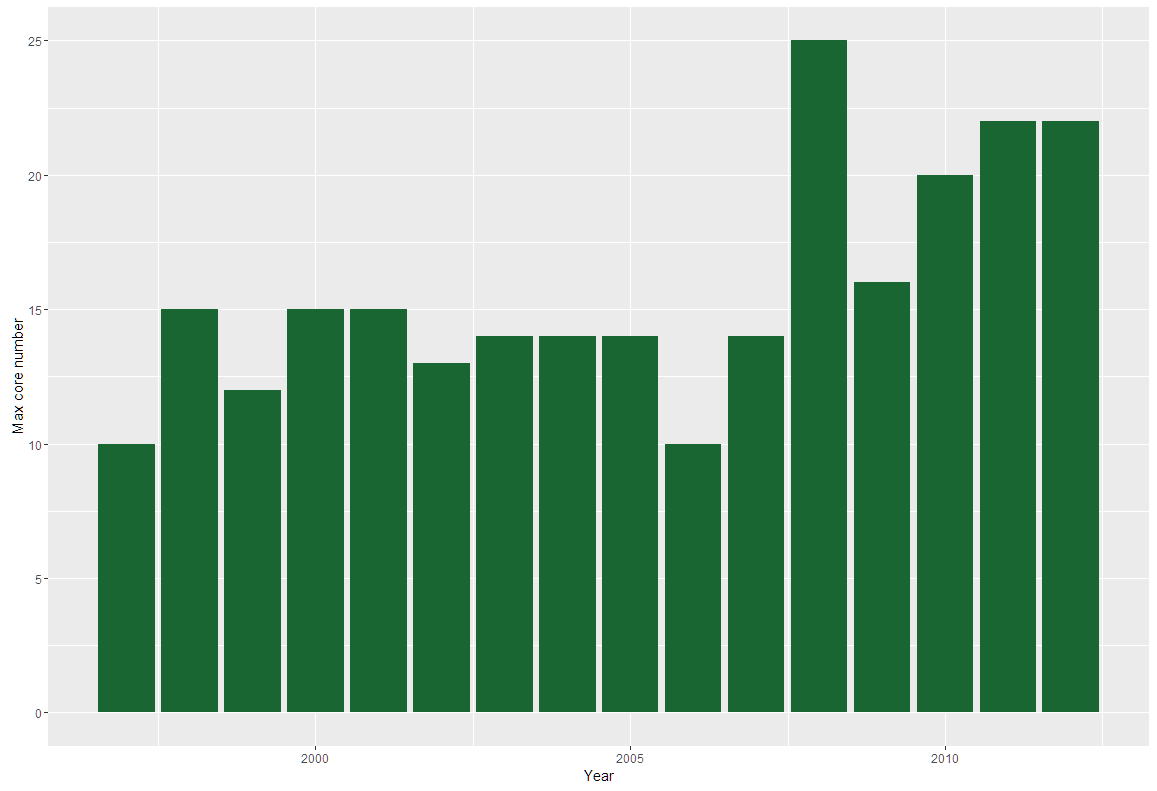
\includegraphics[width=\textwidth]{./pics/StemCellMaxCore.png}
  \caption{Maximum core numbers by years.}
  \label{stemcell}
\end{figure}

p$_S$-core numbers include in the collaboration also a number of articles produced. In Tab.~\ref{stemcellpscore25} are listed nodes with p$_S$-core number at least equal to $25$.

\begin{center}
\begin{longtable}{rlp{8.5cm}}
\caption{Nodes with p$_S$-core numbers at least equal to $25.$}
\label{stemcellpscore25}\\
 \multicolumn{2}{l}{\textbf{Node}} & \textbf{p$_S$-core number} ($\geq 25$) \\
 \endhead
  6 & HUS/SA       &(2008, 2009, 36), (2009, 2010, 26), (2010, 2011, 31), (2011, 2012, 30), (2012, 2013, 38)\\
  9 & UB/B         &(2008, 2009, 36), (2009, 2010, 26), (2010, 2011, 31), (2011, 2012, 55), (2012, 2013, 39)\\
 12 & HVH/B        &(2008, 2009, 26), (2009, 2010, 30), (2010, 2011, 31), (2011, 2012, 46), (2012, 2013, 38)\\
 27 & HISC3/M      &(2008, 2009, 36), (2009, 2010, 30), (2010, 2011, 31), (2011, 2012, 55), (2012, 2013, 41)\\
 32 & HRYC/M       &(2008, 2009, 36), (2009, 2010, 25), (2010, 2011, 30), (2011, 2012, 54), (2012, 2013, 41)\\
 62 & UAM/M        &(2008, 2009, 36), (2009, 2010, 30), (2010, 2011, 31), (2011, 2012, 55), (2012, 2013, 39)\\
 63 & UCM/M        &(2008, 2009, 36), (2009, 2010, 30), (2010, 2011, 31), (2011, 2012, 55), (2012, 2013, 41)\\
 69 & UMA/MA       &(2008, 2009, 36), (2009, 2010, 26), (2010, 2011, 30), (2011, 2012, 32), (2012, 2013, 37)\\
 40 & HCL/B        &(2008, 2009, 36), (2009, 2010, 30), (2010, 2011, 31), (2011, 2012, 55), (2012, 2013, 41)\\
 46 & IDIBAPS/B    &(2008, 2009, 36), (2009, 2010, 30), (2010, 2011, 31), (2011, 2012, 55), (2012, 2013, 41)\\
 48 & HSCSP/B      &(2008, 2009, 36), (2009, 2010, 30), (2010, 2011, 31), (2011, 2012, 55), (2012, 2013, 41)\\
 38 & UV/V         &(2008, 2009, 36), (2009, 2011, 30), (2011, 2012, 55), (2012, 2013, 41)\\
 11 & USAL/SA      &(2008, 2009, 36), (2010, 2011, 31), (2011, 2012, 42), (2012, 2013, 38)\\
 89 & UPF/B        &(2008, 2009, 36), (2010, 2011, 25), (2011, 2012, 34), (2012, 2013, 40)\\
147 & HGM/M        &(2009, 2010, 26), (2010, 2011, 31), (2011, 2012, 42), (2012, 2013, 39)\\
176 & HUVR/SE      &(2008, 2009, 36), (2010, 2011, 31), (2011, 2012, 55), (2012, 2013, 39)\\
 23 & UNAV         &(2008, 2009, 36), (2009, 2010, 30), (2011, 2012, 54), (2012, 2013, 41)\\
 34 & HCL/V        &(2008, 2009, 25), (2010, 2011, 31), (2011, 2012, 34), (2012, 2013, 38)\\
 36 & UAB/B        &(2008, 2009, 36), (2009, 2011, 30), (2011, 2012, 38), (2012, 2013, 37)\\
 58 & HCUN/NA      &(2008, 2009, 25), (2010, 2011, 28), (2011, 2012, 52), (2012, 2013, 41)\\
 72 & HUMV/S       &(2008, 2009, 36), (2010, 2011, 25), (2011, 2012, 55), (2012, 2013, 41)\\
 76 & HULP/M       &(2008, 2009, 36), (2010, 2011, 31), (2011, 2012, 46), (2012, 2013, 39)\\
 80 & HUPLFV/V     &(2008, 2009, 36), (2009, 2010, 30), (2010, 2011, 31), (2011, 2013, 38)\\
 24 & UPV-EHU      &(2008, 2009, 28), (2009, 2010, 30), (2010, 2011, 31)\\
 13 & HNJ/M        &(2008, 2009, 27), (2010, 2011, 30), (2012, 2013, 38)\\
 16 & ICO/CT       &(2008, 2009, 36), (2010, 2011, 31), (2012, 2013, 37)\\
 51 & HBST/B       &(2008, 2009, 25), (2011, 2012, 33), (2012, 2013, 29)\\
  5 & CIC-IBMCC/SA &(2010, 2011, 30), (2011, 2012, 55), (2012, 2013, 41)\\
 93 & CBMSO/M      &(2010, 2011, 30), (2011, 2012, 44), (2012, 2013, 37)\\
109 & HVN/GR       &(2008, 2009, 36), (2011, 2012, 46), (2012, 2013, 35)\\
112 & INCYL        &(2008, 2009, 36), (2010, 2011, 29), (2012, 2013, 32)\\
 53 & H12O/M       &(2008, 2009, 36), (2011, 2012, 33), (2012, 2013, 37)\\
 55 & HUPH/M       &(2010, 2011, 26), (2011, 2012, 34), (2012, 2013, 36)\\
  2 & HCSC/M       &(2010, 2011, 31), (2011, 2012, 32)\\
 35 & HUGTIP/B     &(2010, 2011, 31), (2012, 2013, 32)\\
 37 & US/SE        &(2009, 2010, 30), (2010, 2011, 31)\\
 67 & CIPF/V       &(2008, 2009, 32), (2012, 2013, 32)\\
 73 & UGR/GR       &(2011, 2012, 39), (2012, 2013, 37)\\
  3 & IN/A         &(2008, 2009, 36)\\
 49 & CMRB/B       &(2008, 2009, 28)\\
307 & HVB/LE       &(2010, 2011, 28)\\
 54 & CNB          &(2012, 2013, 41)\\
 57 & HCLB/Z       &(2011, 2012, 30)\\
 81 & HVA/MU       &(2009, 2010, 30), (2012, 2013, 37)\\
 82 & UM/MU        &(2008, 2009, 36)\\
 85 & UA/A         &(2008, 2009, 25)\\
 87 & HUP/M        &(2011, 2012, 47), (2012, 2013, 41)\\
344 & HSO/M        &(2011, 2012, 25)\\
 91 & CIBERNED     &(2012, 2013, 38)\\
289 & HJXXIII/T    &(2008, 2009, 25)\\
 28 & CT/M         &(2010, 2011, 25)\\
101 & HGC/CS       &(2012, 2013, 27)\\
 96 & BACM/GR      &(2011, 2012, 38), (2012, 2013, 37)\\
272 & ULEON/LE     &(2011, 2012, 55), (2012, 2013, 41)\\
357 & HALC/M       &(2010, 2011, 26)\\
102 & USC          &(2011, 2012, 55), (2012, 2013, 41)\\
108 & HGJF/CA      &(2011, 2012, 26)\\
258 & INIA/M       &(2012, 2013, 38)\\
124 & HJC/C        &(2010, 2011, 30), (2011, 2012, 26)\\
 10 & UNIZAR/Z     &(2008, 2009, 36), (2012, 2013, 25)\\
 15 & HSD/PM       &(2010, 2011, 26), (2012, 2013, 27)\\
 17 & HMM/MU       &(2011, 2012, 38)\\
259 & HMS/Z        &(2011, 2012, 34)\\
 20 & UPC/B        &(2012, 2013, 29)\\
 21 & ICREA/B      &(2010, 2011, 31)\\
 22 & HDM/B        &(2008, 2009, 36), (2012, 2013, 38)\\
403 & SERGAS/C     &(2008, 2009, 36)\\
405 & HVC/ZA       &(2009, 2010, 30)\\
133 & HCSOL/MA     &(2012, 2013, 38)\\
134 & IBV/V        &(2008, 2009, 25)\\
135 & CRG/B        &(2008, 2009, 33)\\
535 & SERIDA/O     &(2011, 2012, 34)\\
146 & HSC/GR       &(2010, 2011, 28)\\
149 & IIBM/M       &(2011, 2012, 50)\\
150 & UNIOVI/O     &(2009, 2010, 25), (2010, 2011, 31)\\
153 & UAH/M        &(2008, 2009, 25)\\
171 & UJAEN/J      &(2010, 2011, 25), (2011, 2012, 27)\\
186 & UVA          &(2012, 2013, 27)\\
192 & IRB/B        &(2011, 2012, 38), (2012, 2013, 27)\\
266 & URL/B        &(2012, 2013, 27)\\
 65 & HRS/CO       &(2012, 2013, 32)\\
 66 & HCRUCES/BI   &(2011, 2012, 27)\\
 74 & CIBERDEM     &(2008, 2009, 25)\\
 77 & UPV/V        &(2008, 2009, 28)\\
336 & TERCEL       &(2008, 2009, 25)\\
232 & HUB/B        &(2008, 2009, 36)\\
492 & UPNA/NA      &(2012, 2013, 37)\\
245 & HCAUL/LE     &(2011, 2012, 26)\\
253 & UCLM         &(2011, 2012, 38), (2012, 2013, 32)
\end{longtable}
\end{center}

A diagram of maximum p$_S$-core numbers by year in Fig.~\ref{stemcellps} is great example of collaboration growing with each year. We already noticed that collaborations grew from year 2008 on in Fig.~\ref{stemcell}, but here we see that number of articles in those collaborations also grows.

\begin{figure}[!h]
	\centering
	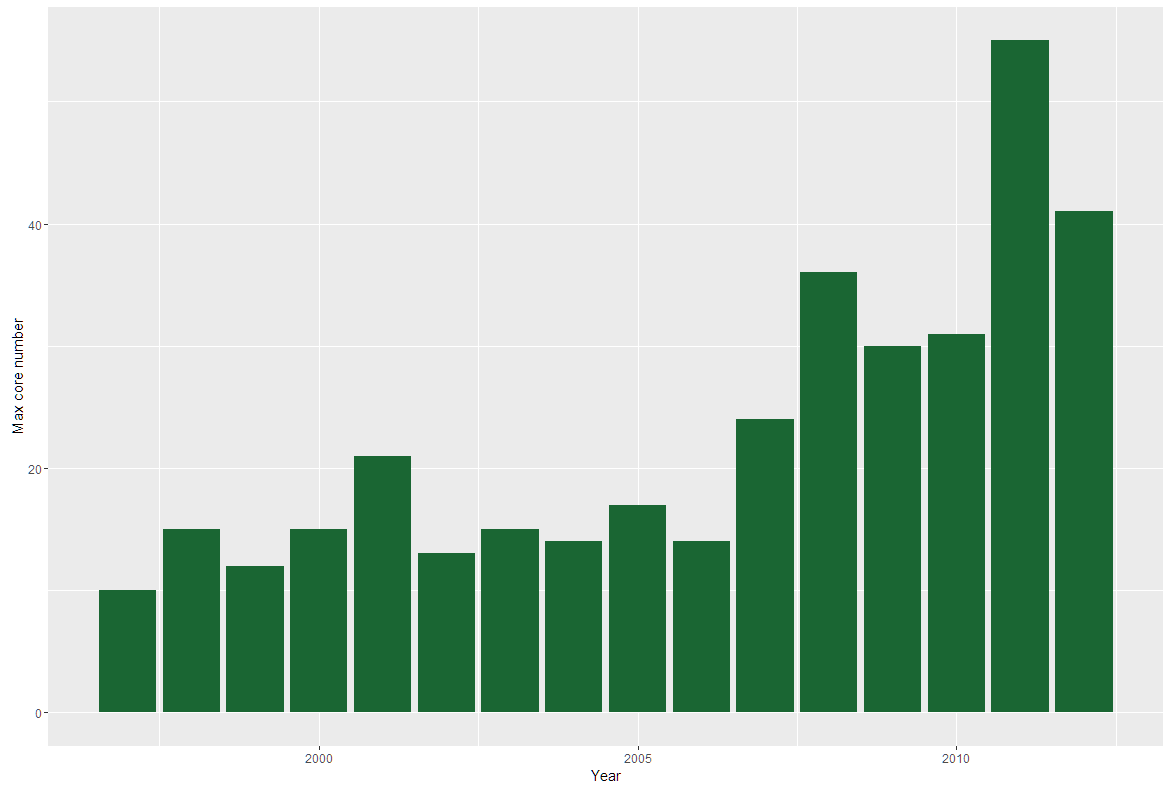
\includegraphics[width=\textwidth]{./pics/maxPsCore.png}
  \caption{Maximum $p_S$-core numbers by years.}
  \label{stemcellps}
\end{figure}


\subsection{Violence network}\footnote{citiraj violencebib, opisi casovno komponento}

Roberto Franzosi collected the data from the journal news in the period from January 1919 to December 1922. He was collecting information about the different types of interactions between political parties and other groups of people in Italy. The violence network contains only the data about violent actions and counts the number of interactions per month.

A network consists of $n = 29$ nodes representing groups of people and $m = 105$ links representing violent interactions.

To see which groups of people were having violent interactions with largest number of other groups we calculated temporal core numbers (see Fig.~\ref{violencecore3}). Maximum core number is $3$ and is present in only $9$ groups, two of which are unknown ("undefined" and "?"). These core numbers appear in months 29, 31, 33, 39, and 40. To see which groups had violent interactions with at least two different groups of people in given month, see Fig.~\ref{violencecore2}.

\begin{center}
\begin{longtable}{rll}
\caption{Nodes with core numbers at least equal to $3.$}
\label{violencecore3}\\
 \multicolumn{2}{l}{\textbf{Node}} & \textbf{Core number} ($\geq 3$)\\
 \endhead
 16 & workers      &(29, 30, 3), (33, 34, 3), (39, 41, 3)\\
  1 & undefined    &(29, 30, 3), (39, 40, 3)\\
  2 & ?            &(31, 32, 3), (33, 34, 3), (40, 41, 3)\\
  3 & people       &(31, 32, 3), (33, 34, 3), (39, 40, 3)\\
  4 & police       &(31, 32, 3), (33, 34, 3), (40, 41, 3)\\
 21 & catholics    &(33, 34, 3)\\
  7 & fascists     &(29, 30, 3), (31, 32, 3), (33, 34, 3), (39, 41, 3)\\
  8 & communists   &(29, 30, 3)\\
 10 & socialists   &(31, 32, 3), (40, 41, 3)
\end{longtable}
\end{center}

\begin{center}
\begin{longtable}{rlp{8.3cm}}
\caption{Nodes with core numbers at least equal to $2.$}
\label{violencecore2}\\
 \multicolumn{2}{l}{\textbf{Node}} & \textbf{Core number} ($\geq 2$)\\
 \endhead
  1 & undefined    &(15, 16, 2), (17, 18, 2), (25, 29, 2), (29, 30, 3), (31, 32, 2), (38, 39, 2), (39, 40, 3),
                    (41, 44, 2), (45, 46, 2), (48, 49, 2)\\
  2 & ?            &(14, 16, 2), (17, 18, 2), (28, 29, 2), (31, 32, 3), (32, 33, 2), (33, 34, 3), (34, 35, 2),
                    (40, 41, 3)\\
  3 & people       &(16, 18, 2), (23, 24, 2), (25, 26, 2), (28, 30, 2), (31, 32, 3), (33, 34, 3), (35, 37, 2),
                    (39, 40, 3), (41, 43, 2), (48, 49, 2)\\
  4 & police       &(11, 12, 2), (14, 20, 2), (21, 23, 2), (29, 31, 2), (31, 32, 3), (32, 33, 2), (33, 34, 3), (34, 37, 2), (38, 40, 2), (40, 41, 3)\\
  5 & land owners  &(15, 16, 2), (17, 20, 2), (29, 30, 2), (36, 37, 2), (38, 40, 2), (42, 43, 2)\\
  7 & fascists     &(11, 12, 2), (16, 17, 2), (19, 20, 2), (21, 24, 2), (25, 29, 2), (29, 30, 3), (30, 31, 2), (31, 32, 3), (32, 33, 2), (33, 34, 3), (34, 37, 2), (38, 39, 2), (39, 41, 3), (41, 44, 2), (45, 46, 2), (48, 49, 2)\\
  8 & communists   &(28, 29, 2), (29, 30, 3), (31, 33, 2), (35, 37, 2), (43, 44, 2)\\
  9 & workers (agr)&(15, 16, 2), (17, 20, 2), (28, 30, 2), (31, 32, 2), (33, 35, 2), (38, 43, 2), (45, 46, 2)\\
 10 & socialists   &(11, 12, 2), (16, 18, 2), (19, 20, 2), (22, 23, 2), (25, 26, 2), (27, 30, 2), (31, 32, 3), (33, 37, 2), (38, 40, 2), (40, 41, 3), (41, 42, 2)\\
 12 & war affected  &(35, 36, 2), (39, 40, 2)\\
 13 & protesters   &(15, 16, 2), (21, 22, 2), (29, 30, 2), (31, 32, 2), (38, 40, 2)\\
 16 & workers      &(11, 12, 2), (14, 18, 2), (19, 20, 2), (21, 24, 2), (25, 26, 2), (27, 29, 2), (29, 30, 3), (30, 33, 2), (33, 34, 3), (34, 37, 2), (38, 39, 2), (39, 41, 3), (41, 44, 2), (45, 46, 2)\\
 17 & the right    &(17, 18, 2), (41, 42, 2)\\
 19 & populars     &(41, 42, 2)\\
 20 & students     &(17, 18, 2)\\
 21 & catholics    &(33, 34, 3)\\
 25 & republicans  &(26, 27, 2)\\
 26 & thugs        &(29, 30, 2)\\
 27 & prisoners/arrested  &(40, 41, 2)
\end{longtable}
\end{center}

A notion of p$_S$-core number tells us overall number of violent interactions in given month - including number of such interactions with each group in the same p$_S$-core. Most violent groups are listed in Tab.~\ref{violencecore10}.

\begin{center}
\begin{longtable}{rlp{8.5cm}}
\caption{Nodes with p$_S$-core numbers at least equal to $10.$}
\label{violencecore10}\\
 \multicolumn{2}{l}{\textbf{Node}} & \textbf{$p_S$-core number} ($\geq 10$)\\
 \endhead
 16 & workers      &(1, 2, 27), (10, 11, 11), (14, 15, 27), (16, 17, 11), (17, 18, 17), (18, 19, 12), (22, 23, 17), (25, 26, 11), (27, 28, 18), (28, 29, 16), (29, 30, 53), (30, 31, 56), (31, 32, 51), (32, 33, 30), 
(33, 34, 17), (34, 35, 71), (35, 36, 76), (36, 37, 53), (37, 38, 11), (38, 39, 23), (39, 40, 54), (40, 41, 13), (41, 42, 174), (42, 43, 25), (43, 44, 20), (45, 46, 15), (46, 47, 25)\\
  1 & undefined    &(25, 26, 11), (27, 28, 12), (28, 29, 16), (41, 42, 133), (45, 46, 11)\\
  3 & people       &(28, 29, 12)\\
  4 & police       &(1, 2, 36), (6, 7, 15), (10, 11, 24), (12, 13, 29), (14, 15, 27), (15, 16, 13), (16, 17, 24), (17, 18, 17), (18, 19, 12), (22, 23, 17), (31, 32, 17)\\
  7 & fascists     &(25, 26, 11), (27, 28, 30), (28, 29, 31), (29, 30, 64), (30, 31, 56), (31, 32, 51), (32, 33, 30), (33, 34, 24), (34, 35, 71), (35, 36, 76), (36, 37, 53), (37, 38, 13), (38, 39, 23), (39, 40, 54), (40, 41, 13), (41, 42, 174), (42, 43, 25), (43, 44, 20), (45, 46, 15), (46, 47, 25)\\
  8 & communists   &(29, 30, 13), (30, 31, 10), (31, 32, 12)\\
  9 & workers (agr)&(10, 11, 24), (16, 17, 24), (28, 29, 16), (30, 31, 13), (36, 37, 11), (39, 40, 15), (43, 44, 10)\\
 10 & socialists   &(10, 11, 10), (12, 13, 29), (27, 28, 30), (28, 29, 31), (29, 30, 64), (30, 31, 29), (31, 32, 17), (32, 33, 14), (33, 34, 24), (34, 35, 38), (35, 36, 23), (36, 37, 26), (37, 38, 13), (38, 39, 19),
         (39, 40, 54), (45, 46, 13)\\
 12 & war affected  &(1, 2, 36)\\
 13 & protesters   &(6, 7, 15), (15, 16, 13), (16, 17, 20)
\end{longtable}
\end{center}

%%%%%%%%%%%%%%%%%%%%%%%%%%%%%
%
%  Conclusion
%
%%%%%%%%%%%%%%%%%%%%%%%%%%%%%
\section{Conclusion}
TODO

Improve the complexity of the algorithm

Extend the algorithm to generalized temporal cores

Find user friendly presentations of results

Compare with the streaming core algorithms

Temporal Quantities - a Python 3 library for temporal network analysis: http://vladowiki.fmf.uni-lj.si/doku.php?id=tq

\textbf{Acknowledgements.}
The second author was partially sponsored by Slovenian Research Agency (ARRS) - projects Z7-7614 (B).


%%%%%%%%%%%%%%%%%%%%%%%%%%%%%%%%%%%%%%%%%%%%%%%%%%%%%%%%%%%%%
%% BIBLIOGRAPHY AND OTHER LISTS
%%%%%%%%%%%%%%%%%%%%%%%%%%%%%%%%%%%%%%%%%%%%%%%%%%%%%%%%%%%%%
%% A small distance to the other stuff in the table of contents (toc)
\addtocontents{toc}{\protect\vspace*{\baselineskip}}

%% The Bibliography
%% ==> You need to run BibTeX for this (Project | Properties... | Uses BibTeX)
%\addcontentsline{toc}{chapter}{Bibliography} %'Bibliography' into toc
\nocite{*} %Even non-cited BibTeX-Entries will be shown.
\bibliographystyle{plain} %Style of Bibliography: plain / apalike / amsalpha / ...
\bibliography{literature}.
\end{document}

